\beginsong{Roter Mond}[
    wuw={Anja Klenk (Hortenring Ernsthofen)}, 
    jahr={1980}, 
    bo={266}, 
    pfii={90}, 
    pfiii={27}, 
    gruen={68}, 
    kssiv={38}, 
    siru={194},
    tonspur={436}, 
]

\beginverse
\endverse
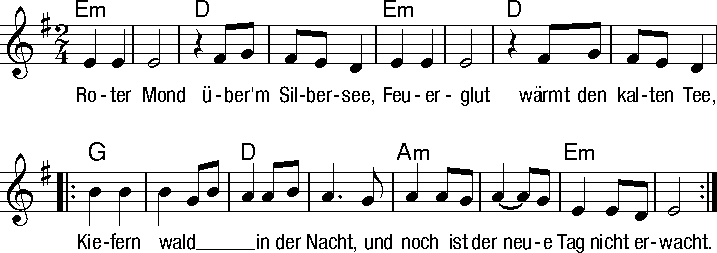
\includegraphics[draft=false, width=1\textwidth]{Noten/Lied078.pdf}	

\beginverse
\[Em]Sterne steh'n \[D]hell am Firmament, \[Em]solche Nacht \[D]findet nie ein End'.
\lrep \[G]Dieses Land, \[D]wild und schön, und \[Am]wir dürfen seine \[Em]Herrlichkeit seh'n. \rrep
\endverse

\beginverse
^Rauher Fels, ^Moos und Heidekraut, ^weit entfernt ^schon der Morgen graut.
\lrep ^Fahne weht, ^weiß und blau, das ^Gras schimmert unterm ^Morgentau. \rrep 
\endverse

\beginverse
\[Em]Fahrt vorbei, \[D]morgen geht es fort. \[Em]Kommen wir \[D]wieder an den Ort?
\[G]Norden ist \[D]unser Glück und \[Am]in uns bleibt nur die Er\[Em]innerung zurück.
\[G]Norden ist \[D]unser Glück und \[Am]wir wünschen uns ein \[Em]neues zurück.
\endverse

\endsong

\beginscripture{}
Dieses Lied ist 1980 bei einem Pfadfinderlager des Hortenring Ernsthofen in Schweden entstanden. Die Farben "weiß und blau" beziehen sich auf das Banner des Pfadfinderbundes. Dieser Bund wurde Ende der Neunziger Jahre aufgelöst.
Wenn der Mond nah am Horizont steht, dann wird das Licht so durch die Atmosphäre gefiltert, dass er rot erscheint.
\endscripture 
